\begin{figure}[ht]
	\centering

%\usetikzlibrary{arrows}
\begin{tikzpicture}

\draw [ultra thick] (-2.5,2.5) rectangle (1.5,-1.5);
\node (v1) at (-7.5,1.5) {};
\node (v2) at (-2.4,1.5) {};
\node (v4) at (-2.4,-0.5) {};
\node (v3) at (-7.5,-0.5) {};
\node (v5) at (1.4,1.5) {};
\node (v6) at (6.5,1.5) {};
\node (v8) at (6.5,-0.5) {};
\node (v7) at (1.4,-0.5) {};
\draw  [->](v1) edge node[above]{\(\bm z_{\ell-1}\)}(v2);
\draw  [<-](v3) edge node[above]{\(\dfrac{\partial L}{\partial \bm z_{\ell-1}}=\dfrac{\partial L}{\partial \bm z_{\ell}}\dfrac{\partial \bm z_{\ell}}{\partial \bm z_{\ell-1}}\)}(v4);
\draw  [->](v5) edge node[above]{\(\bm z_{\ell} = \bm \sigma_{\ell}(\bm z_{\ell-1})\)}(v6);
\draw  [<-](v7) edge node[above]{\(\dfrac{\partial L}{\partial \bm z_{\ell}}\)}(v8);
\node at (-0.5,1.5) {\(\sigma_{\ell} = \bm f_{\ell}(\langle \bm W_{\ell}, \cdot \rangle)\)};
\node at (-0.5,-0.5) {\(\nabla_{\bm W_{\ell}}\sigma_{\ell} = \dfrac{\partial L}{\partial \bm z_{\ell}}\dfrac{\partial \bm z_{\ell}}{\partial \bm W_{\ell}}\)};
\node at (-0.5,3) {Layer $\ell$};
\end{tikzpicture}
	\caption[Conceptualized model of a single network layer.]{A model of a single layer in a neural network. For the feedforward pass it calculates  \(\bm z_{\ell} = \bm \sigma_{\ell}(\bm z_{\ell-1}) = \bm f_{\ell}(\langle \bm W_{\ell},\bm z_{\ell-1}\rangle) \).  On the backward pass it calculates \( \dfrac{\partial L}{\partial \bm W_{\ell}} \) and \( \dfrac{\partial L}{\partial \bm z_{\ell-1}} \). The layer uses \( \dfrac{\partial L}{\partial \bm W_{\ell}} \) to update its own weights with gradient descent. The layer passes \( \dfrac{\partial L}{\partial \bm z_{\ell-1}} \) to the previous layer to use.}
	
\label{fig:backprop}
\end{figure}